\documentclass{beamer}
\usepackage[utf8]{inputenc}
\usepackage{amsmath}
\usepackage{graphicx}

% Title Information
\title[Physics-Constrained Gaussian Splatting]{Research Gaps in Physics-Constrained Gaussian Splatting for Medical Imaging}
\subtitle{Integrating Physical Constraints into 3D Representations}
%\author{Your Name}
%\institute{Your Institution}
\date{\today}

\begin{document}

% Slide 1: Title Slide
\begin{frame}
    \titlepage
\end{frame}

% Slide 2: Agenda
\begin{frame}{Agenda}
    \tableofcontents
\end{frame}

% Slide 3: Background on Gaussian Splatting
\section{Background on Gaussian Splatting}
\begin{frame}{Background on Gaussian Splatting}
    \begin{itemize}
        \item \textbf{Definition:} Explicit 3D representation using a cloud of Gaussians.
        \item \textbf{Advantages:}
        \begin{itemize}
            \item Real-time rendering.
            \item High efficiency compared to NeRF-based methods.
        \end{itemize}
        \item \textbf{Current Applications:}
        \begin{itemize}
            \item RGB novel view synthesis.
            \item Emerging use in X-ray and CT reconstruction.
        \end{itemize}
    \end{itemize}
    \begin{figure}
        \centering
        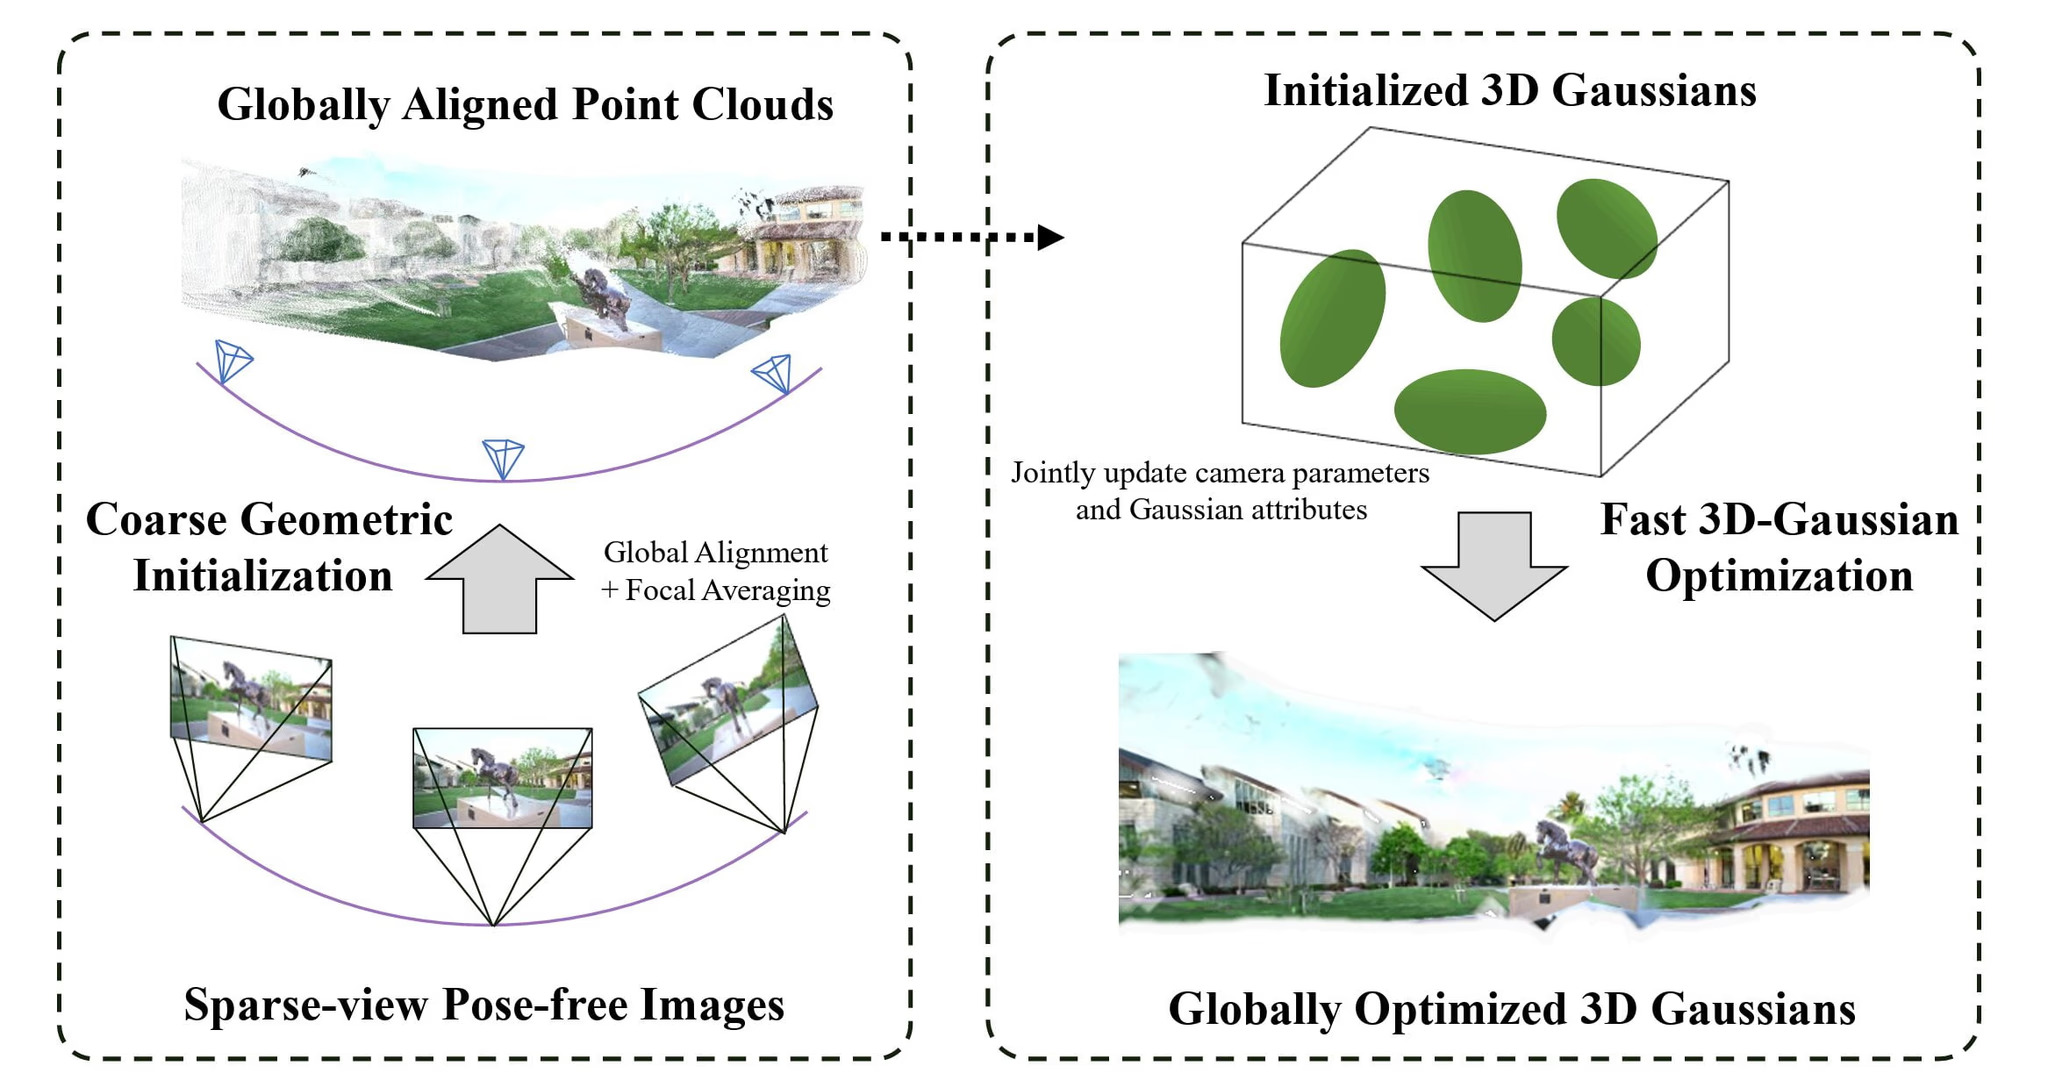
\includegraphics[width=0.6\textwidth]{3DGS.jpg}
        \caption{Illustration of a 3D scene represented by Gaussian splats.}
    \end{figure}
\end{frame}

% Slide 4: Current State-of-the-Art in Medical Imaging
\section{Current State-of-the-Art in Medical Imaging}
\begin{frame}{Current State-of-the-Art in Medical Imaging}
    \begin{itemize}
        \item \textbf{Neural Radiance Fields (NeRF):}
        \begin{itemize}
            \item Implicit representation.
            \item High-quality reconstructions.
            \item Limitations: long training/inference times, heavy computation.
        \end{itemize}
        \item \textbf{Gaussian Splatting (3DGS):}
        \begin{itemize}
            \item Fast and efficient in the RGB domain.
            \item Initial adaptations for X-ray (e.g., X-Gaussian).
        \end{itemize}
        \item \textbf{Key Limitation:} Lack of explicit integration of physical imaging models.
    \end{itemize}
    \begin{table}
        \centering
        \begin{tabular}{|l|c|c|}
            \hline
            \textbf{Method} & \textbf{Training Time} & \textbf{Inference Speed} \\
            \hline
            NeRF & Long & Slow \\
            3DGS & Short & Fast \\
            \hline
        \end{tabular}
        \caption{Comparison of NeRF and 3DGS methods.}
    \end{table}
\end{frame}

% Slide 8: Exploration Direction 2 – Incorporating MRI Signal Models
\section{Exploration Direction 2}
\begin{frame}{Difference between NeRF vs Gaussian Splatting}
    \begin{figure}
        \centering
        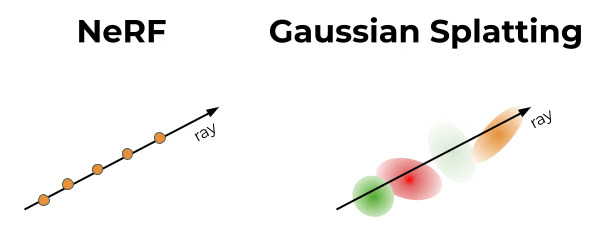
\includegraphics[width=0.95\textwidth]{NeRF vs GS.jpg}
    \end{figure}
\end{frame}


% Slide 5: Identification of the Research Gap
\section{Identification of the Research Gap}
\begin{frame}{Identification of the Research Gap}
    \begin{itemize}
        \item \textbf{The Gap:} Current Gaussian splatting models do not incorporate known physical constraints.
        \item \textbf{Why It Matters:}
        \begin{itemize}
            \item In X-ray imaging: disregard of the Beer–Lambert law (attenuation is not view-dependent).
            \item In MRI: neglect of complex-valued signal formation (T1/T2 relaxations, echo time).
        \end{itemize}
        \item \textbf{Implication:} Reconstructions may be less accurate, less robust, and not interpretable in physical terms.
    \end{itemize}
    \begin{figure}
        \centering
        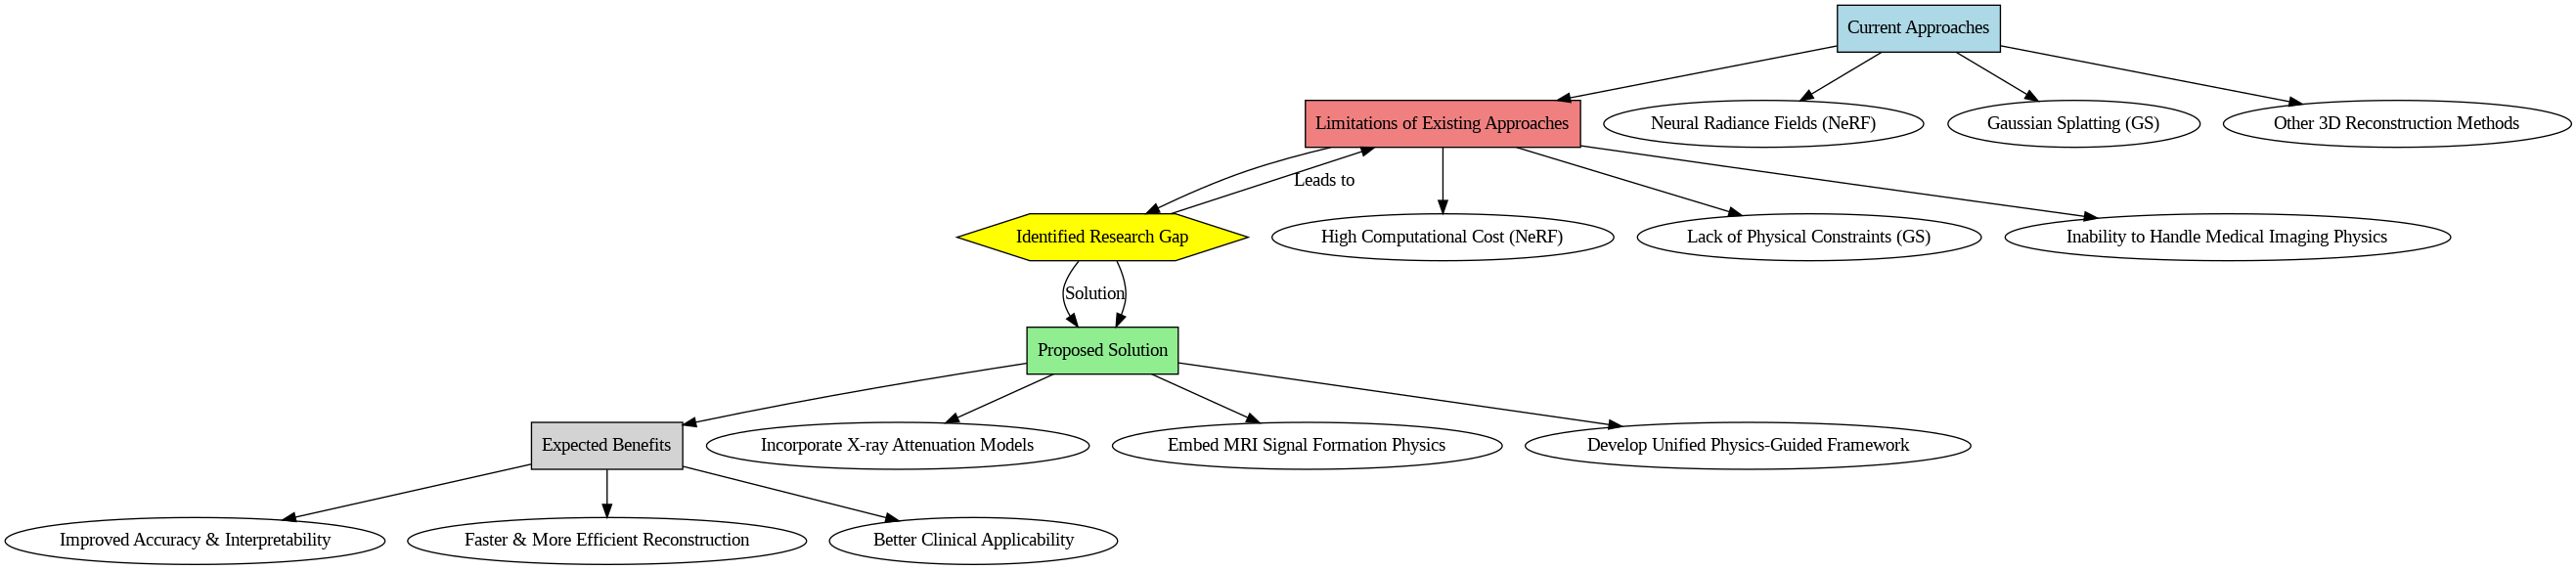
\includegraphics[width=0.8\textwidth]{research_gap_flowchart.png}
    \end{figure}
\end{frame}

% Slide 5: Identification of the Research Gap
\section{Identification of the Research Gap}
\begin{frame}{Identification of the Research Gap}
    \begin{figure}
        \centering
        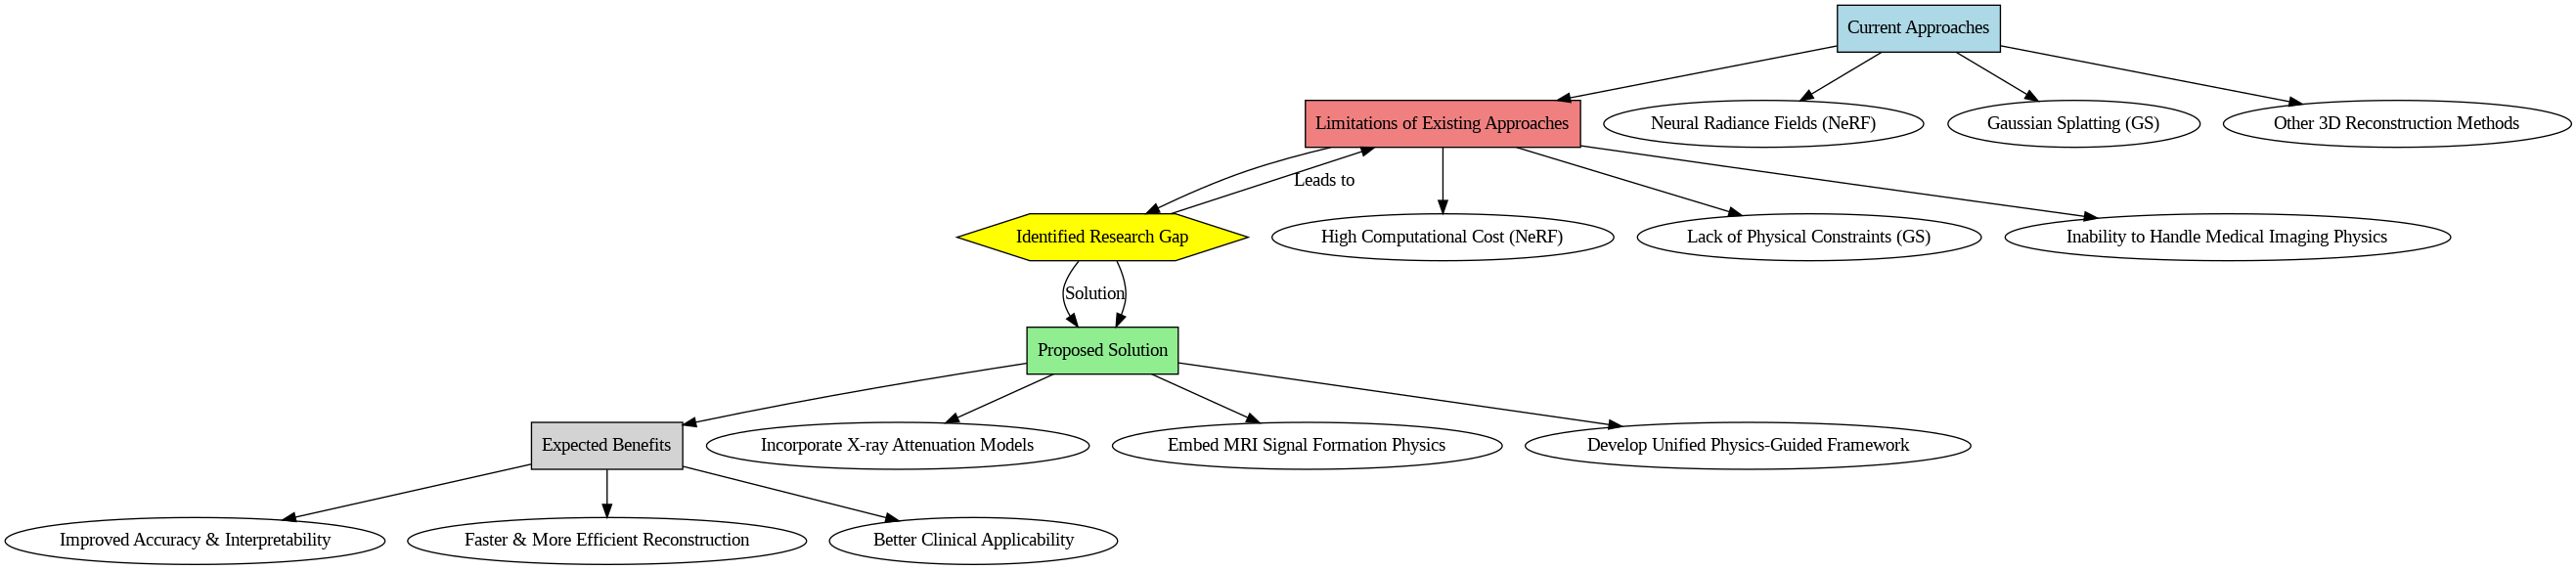
\includegraphics[width=1\textwidth, height=0.5\textwidth]{research_gap_flowchart.png}
    \end{figure}
\end{frame}

% Slide 6: Understanding Physical Constraints
\section{Understanding Physical Constraints}
\begin{frame}{Understanding Physical Constraints}
    \begin{itemize}
        \item \textbf{X-ray Attenuation:}
        \begin{itemize}
            \item Governed by the Beer–Lambert law:
            \[
            I = I_0 \exp\left(-\int_{\text{ray}} \mu(x) \,dx\right)
            \]
            \item \(\mu(x)\) = local attenuation/density.
        \end{itemize}
        \item \textbf{MRI Signal Model:}
        \begin{itemize}
            \item Signal equations depend on proton density and relaxation times (T1, T2).
            \item Complex-valued signals with magnitude and phase.
        \end{itemize}
        \item \textbf{Goal:} Embed these models into the Gaussian splatting framework.
    \end{itemize}
    \begin{figure}
    \centering
    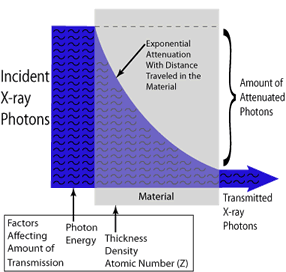
\includegraphics[width=0.4\textwidth, height=0.3\textwidth]{Photon-Absorption.png}
    \caption{Diagrams illustrating X-ray attenuation and MRI signal formation.}
\end{figure}

\end{frame}

% Slide 7: Exploration Direction 1 – Embedding X-ray Attenuation Laws
\section{Exploration Direction 1}
\begin{frame}{Embedding X-ray Attenuation Laws}
    \begin{itemize}
        \item \textbf{Redesigning the Gaussian Kernel:}
        \begin{itemize}
            \item Associate each Gaussian with an attenuation (density) parameter.
            \item Modify the splatting integration to reflect the Beer–Lambert law.
        \end{itemize}
        \item \textbf{Physics-Based Loss Function:}
        \begin{itemize}
            \item Add a loss term measuring the discrepancy between measured X-ray projections and those predicted by integrating Gaussian contributions along rays.
            \item Example loss:
            \[
            \mathcal{L}_{\text{physics}} = \| I_{\text{measured}} - I_0 \exp(-\sum_{i} \mu_i \, w_i) \|_1
            \]
            where \(w_i\) is the weight determined by the Gaussian's contribution along the ray.
        \end{itemize}
        \item \textbf{Expected Outcomes:}
        \begin{itemize}
            \item Improved reconstruction fidelity and physical consistency.
            \item Enhanced robustness under low-dose and sparse conditions.
        \end{itemize}
    \end{itemize}
\end{frame}


% Slide 8: Exploration Direction 2 – Incorporating MRI Signal Models
\section{Exploration Direction 2}
\begin{frame}{Incorporating MRI Signal Models}
    \begin{itemize}
        \item \textbf{Adapting Gaussian Splatting for MRI:}
        \begin{itemize}
            \item Extend the representation to handle complex signals (magnitude and phase).
            \item Assign each Gaussian parameters corresponding to tissue-specific relaxation times (T1, T2).
        \end{itemize}
        \item \textbf{Differentiable MRI Forward Model:}
        \begin{itemize}
            \item Develop a module that simulates the MRI acquisition process (e.g., Fourier sampling, signal decay).
            \item Use the simulated MRI signals as part of the training loss.
        \end{itemize}
        \item \textbf{Potential Benefits:}
        \begin{itemize}
            \item More accurate reconstruction in fast MRI and low-field MRI scenarios.
            \item Enhanced consistency with known tissue properties.
        \end{itemize}
    \end{itemize}
    \begin{figure}
        \centering
        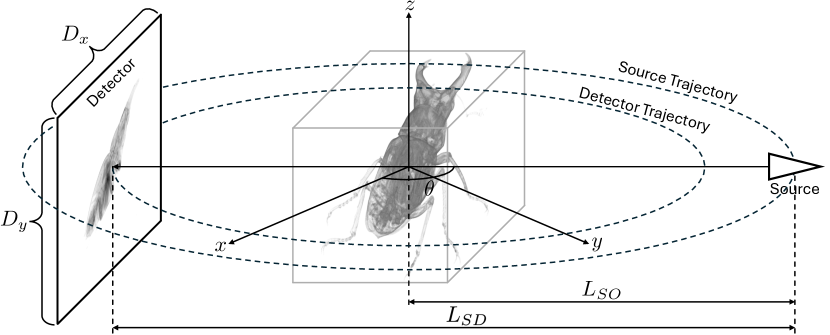
\includegraphics[width=0.6\textwidth]{x9.png}
        \caption{Schematic of possible MRI signal formation and Gaussian splatting integration.}
    \end{figure}
\end{frame}

% Slide 9: Benefits of a Unified, Physics-Constrained Framework
\section{Benefits of a Unified Framework}
\begin{frame}{Benefits of a Unified, Physics-Constrained Framework}
    \begin{itemize}
        \item \textbf{Accuracy \& Robustness:}
        \begin{itemize}
            \item Reconstructions adhere to known physical laws, reducing artifacts and noise.
        \end{itemize}
        \item \textbf{Interpretability:}
        \begin{itemize}
            \item Gaussian parameters (density, relaxation times) correspond to actual physical quantities.
        \end{itemize}
        \item \textbf{Data Efficiency:}
        \begin{itemize}
            \item Leveraging physics reduces the need for vast amounts of data, as the model is partially "pre-informed" by physical priors.
        \end{itemize}
        \item \textbf{Clinical Impact:}
        \begin{itemize}
            \item Potential for lower radiation dose (in CT) and better diagnostic quality.
            \item Improved trust and understanding from clinicians due to interpretable parameters.
        \end{itemize}
    \end{itemize}
    \begin{figure}
        \centering
        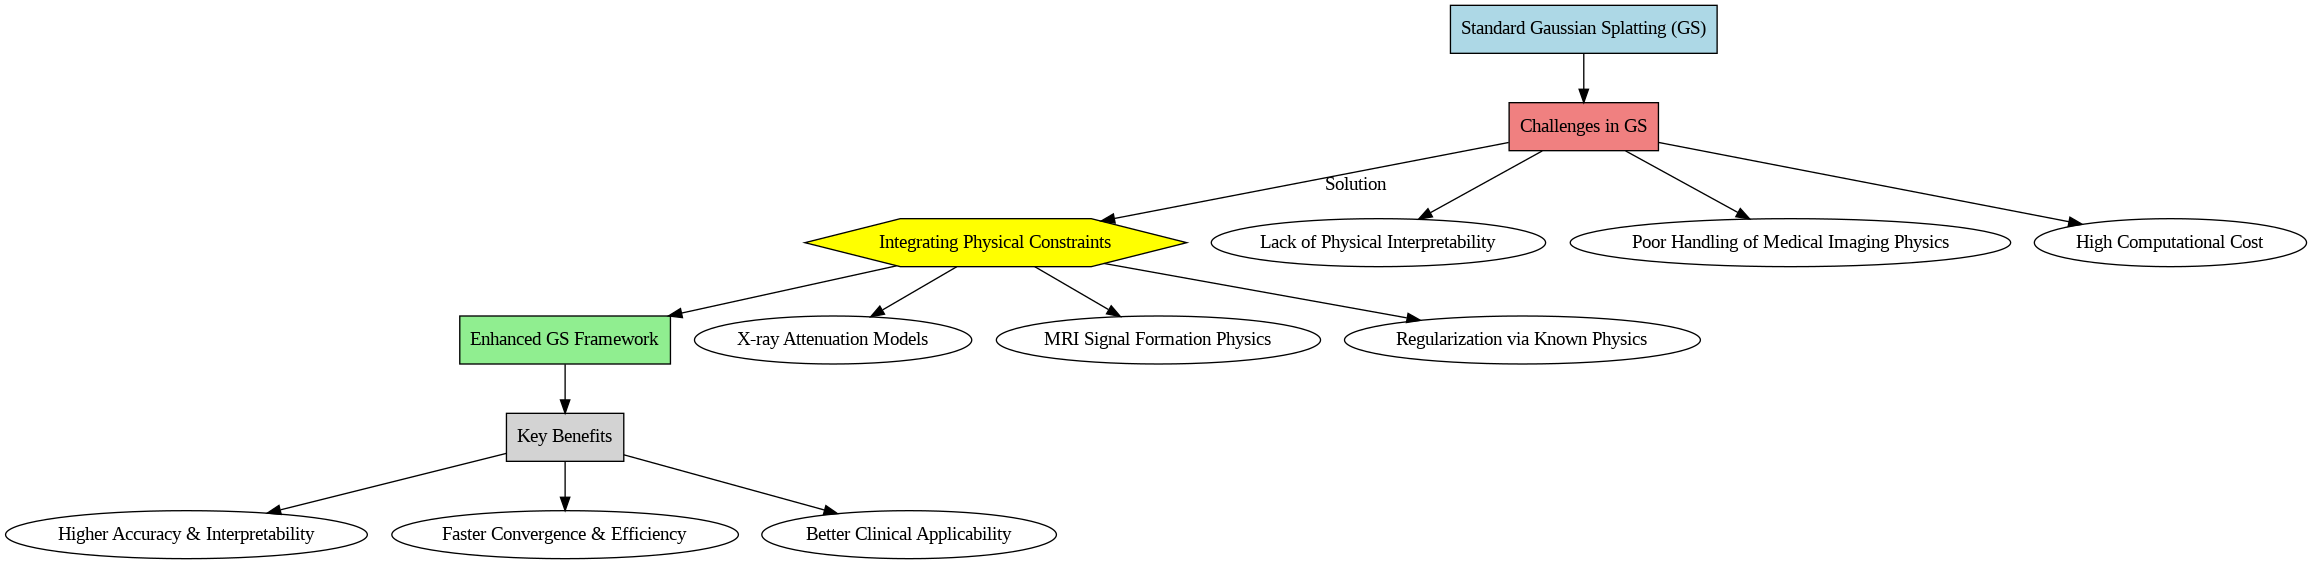
\includegraphics[width=0.8\textwidth]{Untitled.png}
        \caption{Illustration of benefits from integrating physical constraints into Gaussian splatting.}
    \end{figure}
\end{frame}

% Slide 11: Challenges and Future Directions
\section{Challenges and Future Directions}
\begin{frame}{Challenges and Future Directions}
    \begin{itemize}
        \item \textbf{Computational Complexity:}
        \begin{itemize}
            \item Balancing real-time performance with the added computational load from physics-based models.
        \end{itemize}
        \item \textbf{Optimization Stability:}
        \begin{itemize}
            \item Ensuring convergence when incorporating additional physical constraints into the model.
        \end{itemize}
        \item \textbf{Validation:}
        \begin{itemize}
            \item Necessity for extensive validation on diverse clinical datasets to ensure model robustness.
        \end{itemize}
        \item \textbf{Extension to Multimodal Data:}
        \begin{itemize}
            \item Combining data from multiple imaging modalities (e.g., PET/MRI) within a unified framework.
        \end{itemize}
        \item \textbf{Potential Collaborations:}
        \begin{itemize}
            \item Bridging expertise from computer graphics, machine learning, and medical physics to address these challenges.
        \end{itemize}
    \end{itemize}
\end{frame}

% Slide 12: Summary and Conclusion
\section{Summary and Conclusion}
\begin{frame}{Summary and Conclusion}
    \begin{itemize}
        \item \textbf{Recap of the Gap:}
        \begin{itemize}
            \item Current Gaussian splatting methods lack integration of physical imaging models.
        \end{itemize}
        \item \textbf{Proposed Exploration:}
        \begin{itemize}
            \item Embedding X-ray attenuation laws and MRI signal models into the Gaussian splatting framework.
        \end{itemize}
        \item \textbf{Expected Advantages:}
        \begin{itemize}
            \item Achieving higher accuracy, robustness, and interpretability in medical image reconstructions.
        \end{itemize}
        \item \textbf{Future Impact:}
        \begin{itemize}
            \item Potential for improved reconstruction quality with reduced radiation doses and faster inference times.
        \end{itemize}
        \item \textbf{Final Note:}
        \begin{itemize}
            \item Invitation for discussion and feedback on the proposed research directions.
        \end{itemize}
    \end{itemize}
\end{frame}

\end{document}